\documentclass{standalone}
\usepackage{tikz}

\begin{document}
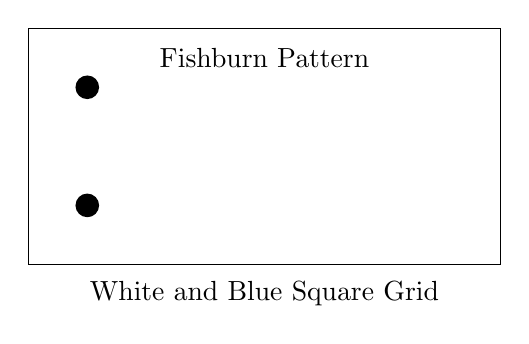
\begin{tikzpicture}[scale=1.5]
    % Draw the grid
    \draw (0,0) rectangle (4,2);
    
    % Fill the dots according to the Fishburn pattern
    \fill[black] (0.5,1.5) circle (0.1); % Top-left square
    \fill[white] (1.5,1.5) circle (0.1); % Top-right square
    \fill[black] (0.5,0.5) circle (0.1); % Bottom-left square
    \fill[white] (1.5,0.5) circle (0.1); % Bottom-right square
    
    % Add labels for clarity
    \node at (2,1.75) {Fishburn Pattern};
    \node at (2,-0.25) {White and Blue Square Grid};
\end{tikzpicture}
\end{document}